\chapter[Metodologia]{Metodologia} \label{metodologia}

A metodologia deste trabalho está dividida em duas seções: a seção \ref{devtools} apresenta as ferramentas que serão utilizadas para realizar a compilação e manipulação dos recursos do jogo (como áudio e imagens) e a seção \ref{devmet} aborda como se darão o desenvolvimento da \textit{engine} e do jogo.

\section{Ferramentas de desenvolvimento} \label{devtools}

  Para a realização do porte do jogo para \textit{Game Boy Advance}, são necessários dois ambientes principais: um ambiente de desenvolvimento onde seja possível implementar o jogo e exportar o binário executável para o console e um ambiente para testar o executável gerado, sendo esse físico ou emulado.

  \subsection{Ambiente de desenvolvimento}

    O jogo foi reescrito utilizando a linguagem C++, na versão 11, pois provê uma série de recursos e estruturas não presentes na linguagem C que facilitarão o desenvolvimento do jogo.

    O ambiente de desenvolvimento utilizado para a implementação do jogo consiste do \textit{kit} de desenvolvimento devkitARM, ferramentas para manipulação das imagens e áudio do jogo.

    \subsubsection{\textit{devkitPro} e \textit{devkitARM}}

      O \texttt{devkitPro}\footnote{\textit{devkitPro}, disponível em \url{https://devkitpro.org/}} é uma organização que provê conjuntos de ferramentas para desenvolvimento de jogos em diversos consoles da \textit{Nintendo}, como \textit{Nintendo GBA}, \textit{Nintendo Wii}, \textit{Nintendo Switch}, dentre outros.

      Dentre esses conjuntos de ferramentas encontra-se o \textit{devkitARM}, \textit{toolchain} que contém o ambiente de desenvolvimento necessário para realizar a compilação do código escrito em C/C++ para a arquitetura de processadores ARM existente no GBA, citado na Seção \ref{gba} do Capítulo \ref{fundamentacao}.

    \subsubsection{Manipulação de imagens e áudio}

      Para o ajuste das imagens do jogo para a resolução de tela do GBA, foi utilizada a ferramenta de manipulação de imagens GIMP\footnote{GNU Image Manipulation Program, disponível em \url{https://www.gimp.org/}}, versão 2.8.

      Para realizar a conversão das imagens para um formato legível no GBA, foi utilizada uma biblioteca C chamada GRIT\footnote{\textit{GBA Raster Image Transmogrifier}, disponível em \url{http://www.coranac.com/projects/grit/}}, versão \texttt{0.8.15}.

      Para a manipulação do áudio do jogo foram utlizadas três ferramentas: \texttt{avconv}\footnote{\texttt{avconv}, disponível em \url{https://github.com/libav/libav}} \texttt{13\_dev0-1601-g56f5018} e \texttt{librosa}\footnote{\texttt{librosa}, disponível em \url{https://github.com/librosa/librosa}} \texttt{0.6.2} para \textit{downsampling} das músicas; e \texttt{modplug tracker}\footnote{\textit{Open Modplug Tracker}, disponível em \url{http://openmpt.org/features}} \texttt{1.27.11.00} para realizar a conversão das músicas para \texttt{.mod}.

  \subsection{Ambiente de teste}

      Para a realização de testes com os executáveis gerados pelo \textit{devkitARM} foi utilizado o emulador de \textit{Game Boy Advance} \textit{VisualBoyAdvance-M}\footnote{\textit{VisualBoyAdvance-M}, disponível em \url{https://github.com/visualboyadvance-m/visualboyadvance-m}}, versão \texttt{2.0.1}.

      O \textit {console} utilizado como ambiente de testes real é um \textit{Nintendo DS}\footnote{\textit{Nintendo DS}, disponível em \url{https://www.nintendo.com/consumer/systems/selectds.jsp}}, que possui um \textit{slot} para cartuchos de \textit{Game Boy Advance}. Neste trabalho foi utilizado um cartucho especial onde é possível escrever arquivos executáveis diretamente nele.

      Para a escrita dos arquivos executáveis neste cartucho foi utilizado o dispositivo \textit{EZFlash II}\footnote{\textit{EZ Flash II}, disponível em \url{http://www.ezfadvance.com/cards/EZ-Flash_2.htm}}. Como essa é uma versão antiga do produto, é necessário instalar um cliente para \textit{upload} dos arquivos para o cartucho. Este cliente só possui compatibilidade com \textit{Windows XP}\footnote{\textit{Windows XP}, disponível em \url{https://support.microsoft.com/pt-br/help/14223/windows-xp-end-of-support}}, fazendo com que seja necessário instalar uma máquina virtual com o sistema operacional.

\section{Metodologia de desenvolvimento} \label{devmet}

  \subsection{Desenvolvimento da \textit{Engine}}

    Para contribuir com uma arquitetura mais manutenível, foi optado por desacoplar a \textit{engine} do jogo em si. A \textit{engine} ficará responsável por implementar os módulos genéricos do jogo, enquanto que o jogo em si conterá as funcionalidades mais específicas.

    A \textit{engine} contém uma classe que representa um objeto do jogo (do inglês, \textit{game object}). Esta classe foi responsável por conter o comportamento genérico de um objeto dentro do jogo (podendo este ser um personagem, uma plataforma, um item coletável, etc.). Ele foi representado de acordo com a Figura \ref{game-object}:

    \vspace{\onelineskip}

    \begin{figure}[H]
      \centering 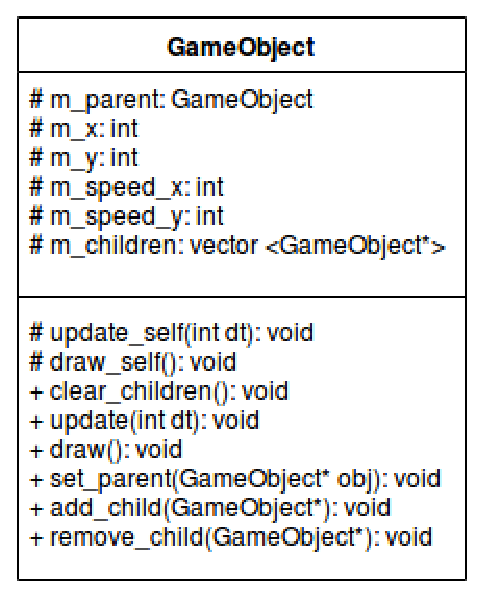
\includegraphics[keepaspectratio=true,scale=0.6]{figuras/game-object.eps}
      \caption[Modelagem da classe \textit{GameObject}]
        {Modelagem da classe \textit{GameObject}.}
      \label{game-object}
    \end{figure}

    Onde os métodos \texttt{update\_self()} e \texttt{draw\_self()}, abstratos, tratam de atualizar o objeto a cada frame e renderizar o objeto na posição \texttt{(x, y)}, respectivamente.

    É importante frisar que os métodos \texttt{update\_self()} e \texttt{draw\_self()} são abstratos e, considerando que o jogo foi portado utilizando C++, estes métodos devem ser puramente virtuais, pois isso garante que qualquer classe que venha a extender de \texttt{GameObject} seja obrigada a implementer suas próprias rotinas específicas de atualização e renderização.

    Além da classe \texttt{GameObject}, os principais componentes da \textit{engine} implementados foram: módulo de vídeo, módulo de áudio, módulo de física e módulo de \textit{input}.

    \subsubsection{Módulo de vídeo}

      O módulo de vídeo foi responsável por renderizar qualquer tipo de imagem e animação existente. Ele contém as seguintes funcionalidades:

      \begin{itemize}
        \item renderizar de um a até quatro imagens de fundo;
        \item renderizar uma ou mais \textit{sprites};
        \item renderizar uma animação (como uma série de \textit{sprites});
        \item movimentar horizontalmente qualquer imagem de fundo (\textit{horizontal scroll});
        \item remover uma imagem, \textit{sprite} ou animação que esteja renderizado da tela;
        \item atualizar a renderização a cada frame, levando em consideração as posições \textit{x} e \textit{y} da \textit{sprite} ou animação; e
        \item configurar a prioridade de exibição de texturas (animações ou \textit{sprites})
      \end{itemize}

      Deve-se lembrar que as imagens renderizadas foram ajustadas para a resolução e formato de cores corretos do GBA.

    \subsubsection{Módulo de áudio}

      O módulo de áudio foi responsável por executar, no momento correto, qualquer música de fundo e efeito sonoro do jogo. Ele contém as seguintes funcionalidades:

      \begin{itemize}
        \item iniciar a execução de uma música de fundo; e
        \item parar a execução de uma música de fundo.
      \end{itemize}

    \subsubsection{Módulo de física}

      O módulo de física teve como principal responsabilidade a detecção de colisões entre objetos do jogo. Ele contém as seguintes funcionalidades:

      \begin{itemize}
        \item simular, opcionalmente, a ação da gravidade em qualquer objeto do jogo;
        \item detectar, opcionalmente, colisões entre todos os objetos do jogo; e
        \item detectar, opcionalmente, colisões entre um objeto e todos os outros objetos do jogo.
      \end{itemize}

    \subsubsection{Módulo de \textit{input}}

      O módulo de \textit{input} foi responsável por receber qualquer pressionamento de qualquer um dos 10 botões e teclas do GBA. Ele tem como funcionalidades:

      \begin{itemize}
        \item detectar se determinado botão foi pressionado; e
        \item detecter se determinado botão está sendo pressionado.
      \end{itemize}

  \subsection{Desenvolvimento do jogo}

    A implementação do jogo foi baseada em classes e foi modelado como mostrado na Figura \ref{model-final}. O personagem principal, os itens coletáveis e plataformas foram representados como \textit{game objects} e também herdam da classe \texttt{Collidable}, para que possam colidir entre si. Já os níveis do jogo são representados pela classe \texttt{TWLevel} e esta, por sua vez, herda da classe \texttt{Level}, que contém a generalização de um nível no jogo. Por fim, a classe \texttt{TWGame} tem como responsabilidade iniciar e realizar a transição entre os níveis do jogo.

    \begin{figure}[H]
      \centering 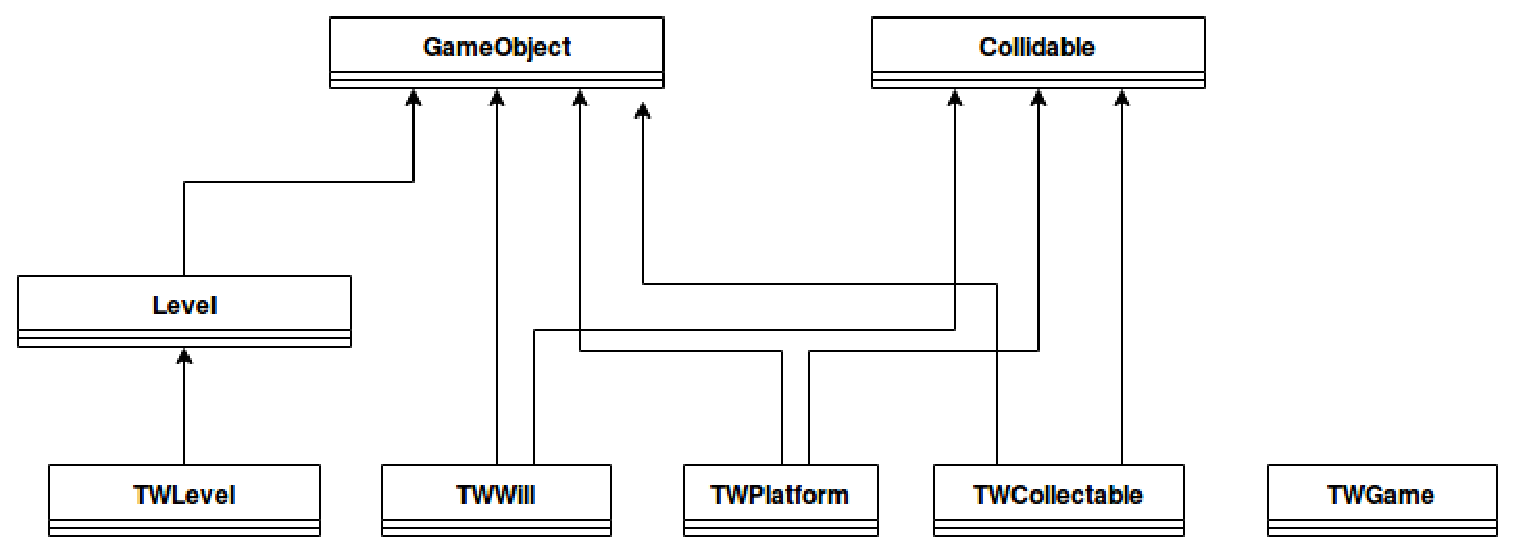
\includegraphics[keepaspectratio=true,scale=0.6]{figuras/modelagem-final.eps}
      \caption[Modelagem dos objetos do jogo]
        {Modelagem dos objetos do jogo.}
      \label{model-final}
    \end{figure}

    Os recursos como imagens e músicas precisaram ser editados para que pudessem ser carregados em memória e utilizados no GBA. No caso das imagens, por exemplo, foram modificadas características como dimensões e quantidade de cores a fim de diminuir seu tamanho para que possam ser convertidas para um formato utilizável no GBA. Já no caso dos arquivos de áudio, a principal mudança realizada foi a diminuição da frequência das músicas, como será explicado na Seção \ref{adapmusic}.